
\chapter{マルクス主義}


\section{『共産党宣言』 (1848)}


典拠:マルクス/エンゲルス、大内兵衛・向坂逸郎訳(1971)『共産党宣言』岩波書店

\subsection{}


今日までのあらゆる社会の歴史は、階級闘争の歴史である。

自由民と奴隷、都市貴族と平民、領主と農奴、ギルドの親方と職人、要するに圧制者と被圧制者はつねにたがいに対立して、ときには暗々のうちに、ときには公然と、不断の闘争をおこなってきた。この闘争はいつも、全社会の革命的改造をもって終るか、そうでないときには相闘う階級の共倒れをもって終った。

歴史の早い諸時期には、われわれは、ほとんどどこでも社会が種々の身分に、社会的地位のさまざまの段階に、完全にわかれているのを見出す。古ローマにおいては、都市貴族、騎兵、平民、奴隷に、中世においては、封建君主、家臣、ギルド組合員、職人、農奴にわかれていた。なおそのうえ、これらの階級の一つ一つのなかが、たいていまた別々の階層にわかれていた。
封建社会の没落から生れた近代ブルジョア社会は、階級対立を廃止しなかった。この社会はただ、あたらしい階級を、圧制のあたらしい条件を、闘争のあたらしい形態を、旧いものとおきかえたにすぎない。

しかしわれわれの時代、すなわちブルジョア階級の時代は、階級対立を単純にしたという特徴をもっている。全社会は、敵対する二大陣営、たがいに直接に対立する二大階級{\——}ブルジョア階級とプロレタリア階級に、だんだんとわかれていく。(38-40)


  \begin{figure}[htbp]
    \centering
      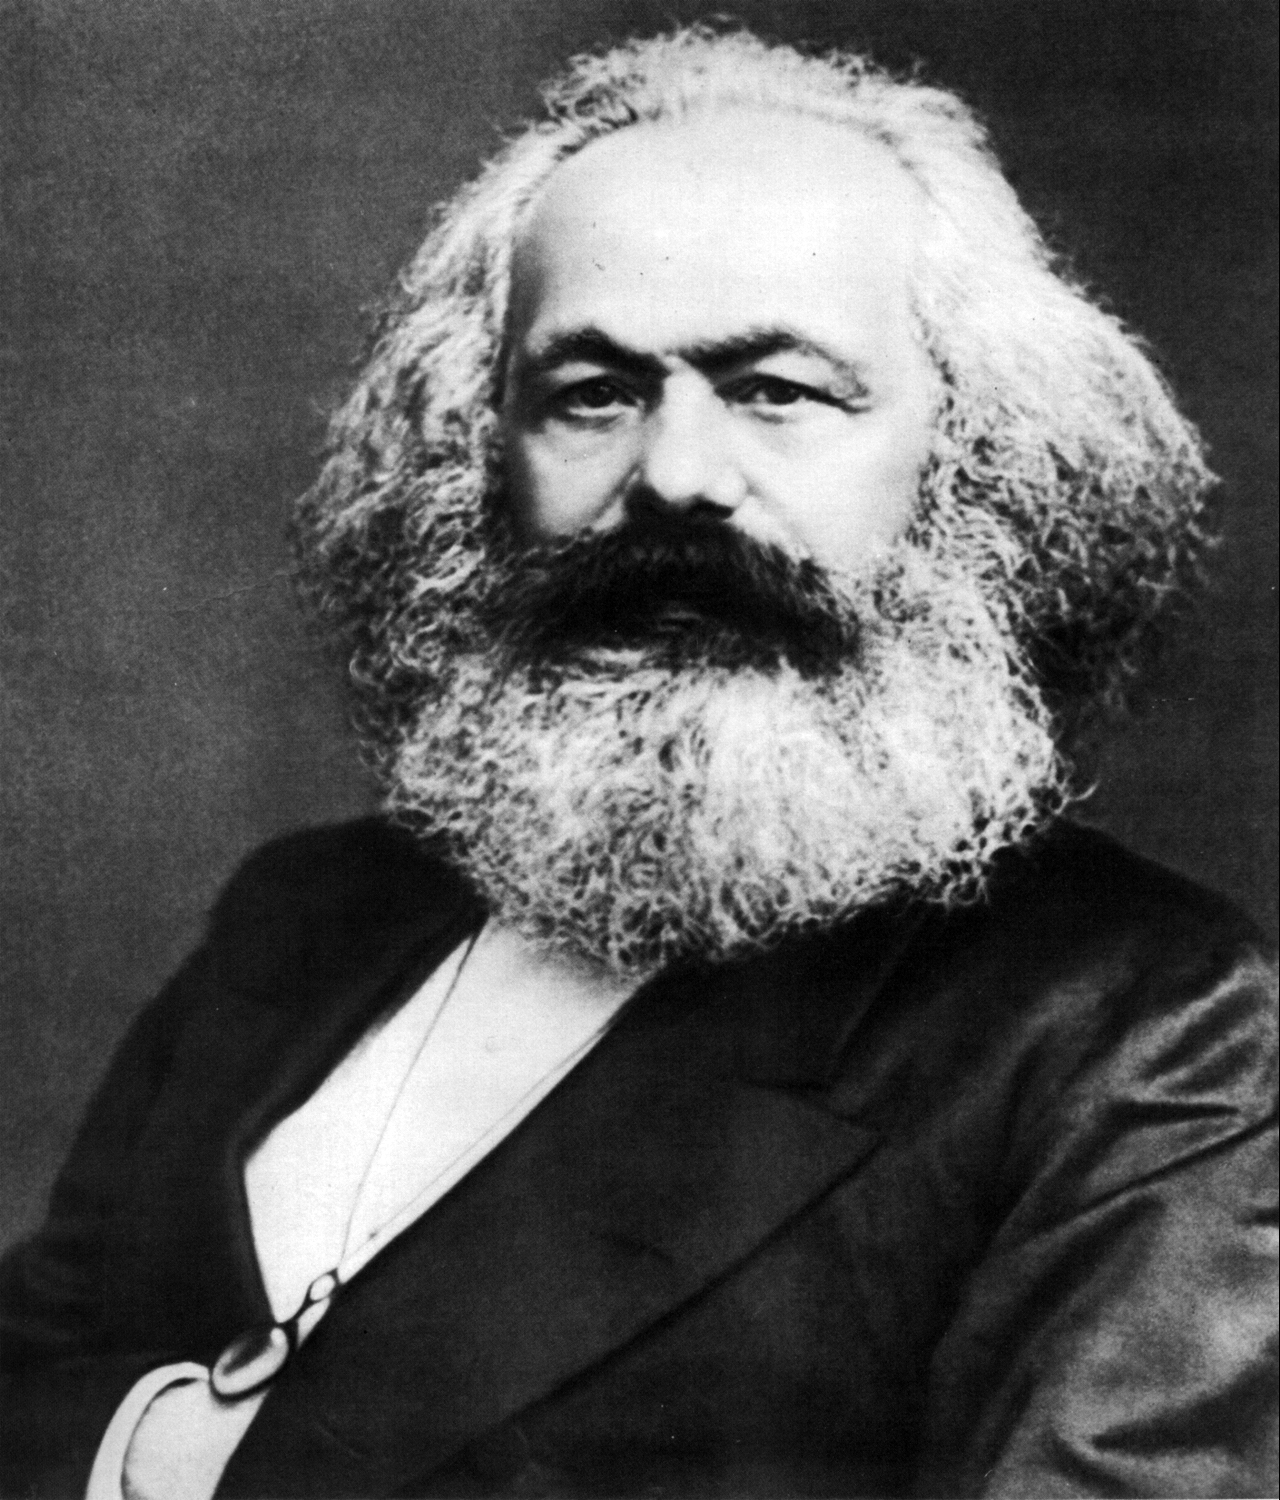
\includegraphics[width=50mm]{images/Karl_Marx.jpg}
      \caption{マルクス} 
  \end{figure}



\subsection{}



ブルジョア階級は、かれらの百年にもみたない階級支配のうちに、過去のすべての世代を合計したよりも大量の、また大規模な生産諸力を作り出した。自然力の征服、機械装置、工業や農業への化学の応用、汽船航海、鉄道、電信、全大陸の耕地化、河川の運河化、地から湧いたように出現した全人口{\——}これほどの生産諸力が社会的労働のふところのなかにまどろんでいたとは、以前のどの世紀が予感しただろうか?

だが、われわれが知ったことは、ブルジョア階級の成長の土台をなす生産手段や交通手段は、封建社会のなかで作られたということである。この生産手段と交通手段の発展がある段階に達すると、封建社会の生産や交換がおこなわれていた諸関係、農業と工場手工業(マニュファクチャ)の封建的体制、一言でいえば封建的所有関係は、そのときまでに発展した生産諸力にもはや適合しなくなった。それは、生産を促進しないで、阻害するようになった。それはいずれもみな変じて足かせとなった。それは粉砕されねばならなかった、そして粉砕された。

それに代って自由競争があらわれた。これにともなって、それに適合した社会的ならびに政治的制度があらわれ、ブルジョア階級の経済的ならびに政治的支配があらわれた。

われわれの眼のまえに、その同じ運動が進行している。ブルジョア的生産ならびに交通諸関係、ブルジョア的所有諸関係、かくも巨大な生産手段や交通手段を魔法で呼び出した近代ブルジョア社会は、自分が呼び出した地下の悪魔をもう使いこなせなくなった魔法使いに似ている(45-46)


\subsection{}


ブルジョア階級が封建制を打ち倒すのに用いた武器は、いまやブルジョア階級自身に向けられる。

しかしブルジョア階級は、みずからに死をもたらす武器をきたえたばかりではない。かれらはまた、この武器を使う人々をも作り出した{\——}近代的労働者、プロレタリアを。(48)

\subsection{}


以前のすべての階級は、支配を獲得したばあい、全社会を自分の生業の諸条件に服従させ、それによって、かれらの既得の生活上の地位を確保しようとつとめた。プロレタリアは、自分自身のこれまでの獲得様式を、したがってまたこれまでの全獲得様式を廃止しなくては、社会的生産諸力を奪取することはできない。プロレタリアは確保すべき自分のものを何ももたない、かれらが破壊しなければならないものは、これまでのすべての私的安全や私的保証である。
これまでのいっさいの運動は、少数者の運動、あるいは少数者の利益のための運動であった。プロレタリアの運動は、途方もない多数者の利益のための、途方もない多数者の独立的運動である。現代社会の最下層であるプロレタリア階級が起きあがり、立ちあがることができるためには、公的社会を形成する階層の全上部構造を空中にけし飛ばさなければならない。(54)

\subsection{}


われわれがすでに見たように、これまでのすべての社会は、圧迫する階級と圧迫される階級との対立のうえに立っていた。しかし一つの階級を圧迫できるためには、その圧迫される階級に、少くとも奴僕的存在ぐらいは保っていけるだけの条件が確保されていなければならない。小市民は封建制的絶対主義の抑圧のもとで努力してブルジョアになった。それと同じように、農奴は農奴制のもとで、努力して自治体(コンミューン)の成員になった。これに反して近代の労働者は、工業の進歩とともに向上する代りに、かれら自身の階級の諸条件を下まわってますますそれ以下に沈んでいく。労働者は貧窮者となり、貧窮は人口や富よりもっと急速に発展する。このことから明らかにわかることは、ブルジョア階級がもうこれ以上社会の支配階級としてとどまる能力をもたず、自分の階級の生存条件を、規制的法則として社会に強制する能力をもたないということである。かれらは支配する能力をもたない、なぜならかれらは、その奴隷に奴隷制の内部においてさえ生存を保証する能力をもたないからであり、またかれらが奴隷から養われる代りに奴隷を養わねばならない状態にまで、その奴隷をおとさざるをえないからである。社会はもはや、ブルジョア階級のもとでは生存することができない。すなわち、ブルジョア階級の生存はもはや社会と相容れないのである。

ブルジョア階級の存在と支配にとってもっとも本質的な条件は、私人の手中への富の集積、すなわち資本の形成と増殖である。資本の条件は賃金労働である。賃金労働はもっぱら労働者相互のあいだの競争にもとづく。工業の進歩の無意志無抵抗な担い手はブルジョア階級であるが、この進歩は、競争による労働者の孤立化の代りに、結合による労働者の革命的団結を作り出す。だから、大工業の発展とともに、ブルジョア階級の足もとから、かれらに生産させ、また生産物を取得させていた土台そのものが取り去られる。かれらは何よりも、かれら自身の墓掘人を生産する。かられの没落とプロレタリア階級の勝利は、ともに不可避である。(55-56)


\subsection{}


共産主義者はだれからも、社会的生産物を取得する権力を奪わない。ただ、この取得によって他人の労働を自分に従属させる権力を奪うだけである。
私有財産の廃止とともに、すべての活動がやみ、一般的怠惰がはびこるであろう、という異論がある。

この考えにしたがえば、ブルジョア社会は、怠惰のためにとうの昔に破滅していたにちがいない。なぜなら、この社会では、働くものは儲けない、儲けるものは働かない、からである。こういう疑念はすべて、資本がなくなれば賃金労働もまたなくなる、という自明のことを他の言葉でいい直しただけである。

物質的生産物の共産主義的取得様式および生産様式に対してなされるすべての非難は、同様に精神的生産物の取得および生産にまで及ぼされる。ブルジョア階級にとって階級的財産の終りが生産自身の終りであるように、階級的教養の終りは、かれらにとって、教養一般の終りと同意義である。

ブルジョアがその失われるのを惜しんでいる教養とは、非常な多数者にとっては、機械になるための修養である。(62)

\subsection{}


思想の歴史の証明するところは、精神的生産は物質的生産とともに作り変えられるということのほかに何があろうか? ある時代の支配的思想は、つねに支配階級の思想にすぎないのである。(66)

\subsection{}


プロレタリア階級は、その政治的支配を利用して、ブルジョア階級から次第にすべての資本を奪い、すべての生産用具を国家の手に、すなわち支配階級として組織されたプロレタリア階級の手に集中し、そして生産諸力の量をできるだけ急速に増大させるであろう。
このことは、もちろんなによりも、所有権への、またブルジョア的生産諸関係への専制的干渉なくしてはできようがない。したがって、その方策は、経済的には不充分で不安定に見えるが、運動が進行するにつれて、自分自身を乗り越えてすすみ、全生産様式の変革への手段として不可避なものとなる。
この方策は、もちろん、それぞれ国が異なるにしたがって異なるであろう。
とはいえ、もっとも進歩した国々にとっては、次の諸方策はかなり一般的に適用されるるであろう。

一、土地所有を収奪し、地代を国家支出に振り向ける。/二、強度の累進税。/三、相続権の廃止。/四、すべての亡命者および反逆者の財産の没収。/五、国家資本および排他的独占をもつ国立銀行によって、信用を国家の手に集中する。/六、すべての運輸機関を国家の手に集中する。/七、国有工場、生産用具の増加、共同計画による土地の耕地化と改良。〔……〕
発展の進行につれて、階級差別が消滅し、すべての生産が結合された個人の手に集中されると、公的権力は政治的性格を失う。本来の意味の政治的権力とは、他の階級を抑圧するための一階級の組織された権力である。プロレタリア階級が、ブルジョア階級との闘争のうちに必然的に階級にまで結集し、革命によって支配階級となり、支配階級として強力的に古い生産諸関係を廃止するならば、この生産諸関係の廃止とともに、プロレタリア階級は、階級対立の、階級一般の存在条件を、したがって階級としての自分自身の支配を廃止する。

階級と階級対立をもつ旧ブルジョア社会の代りに、一つの協力体があらわれる。ここでは、ひとりひとりの自由な発展が、すべての人々の自由な発展にとっての条件である。(68-69)


\newpage{}

\section{エンゲルス『家族・私有財産・国家の起源』 (1884)}



典拠:エンゲルス、戸原四郎訳(1965)『家族・私有財産・国家の起源』岩波書店

\subsection*{}


 % \begin{wrapfigure}{r}{60mm}
 %   \begin{center}
 %     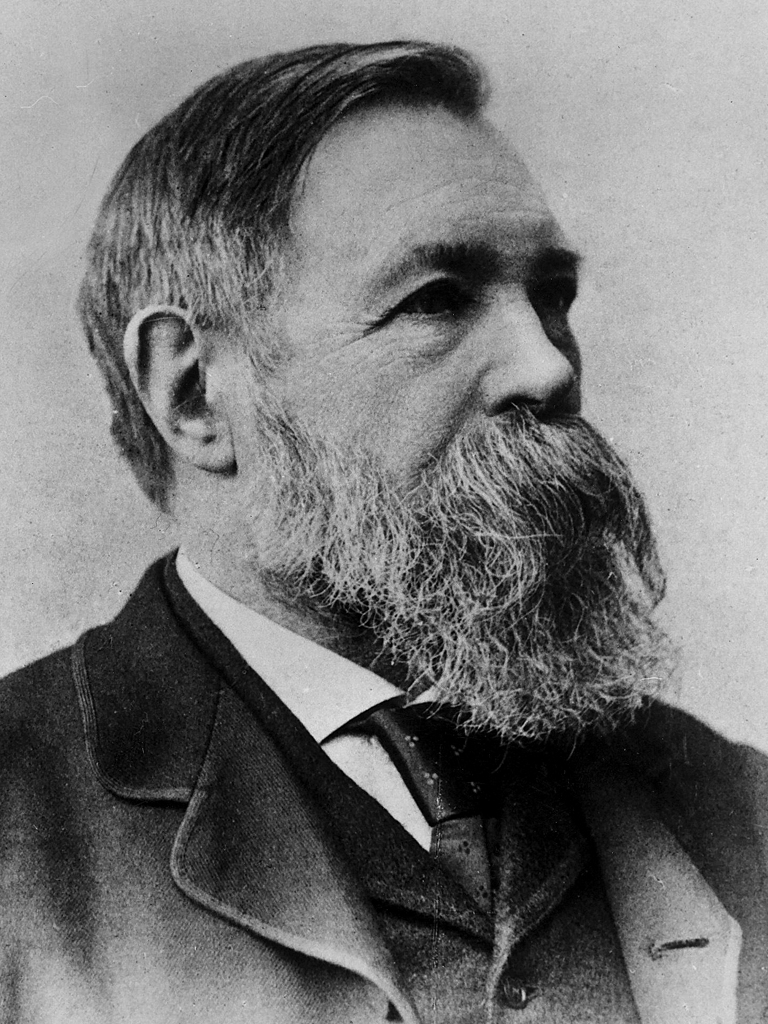
\includegraphics[width=50mm]{images/engels.jpg}
 %     \caption{ホッブズ} 
 %   \end{center}
 % \end{wrapfigure}


  \begin{figure}[htbp]
    \centering
      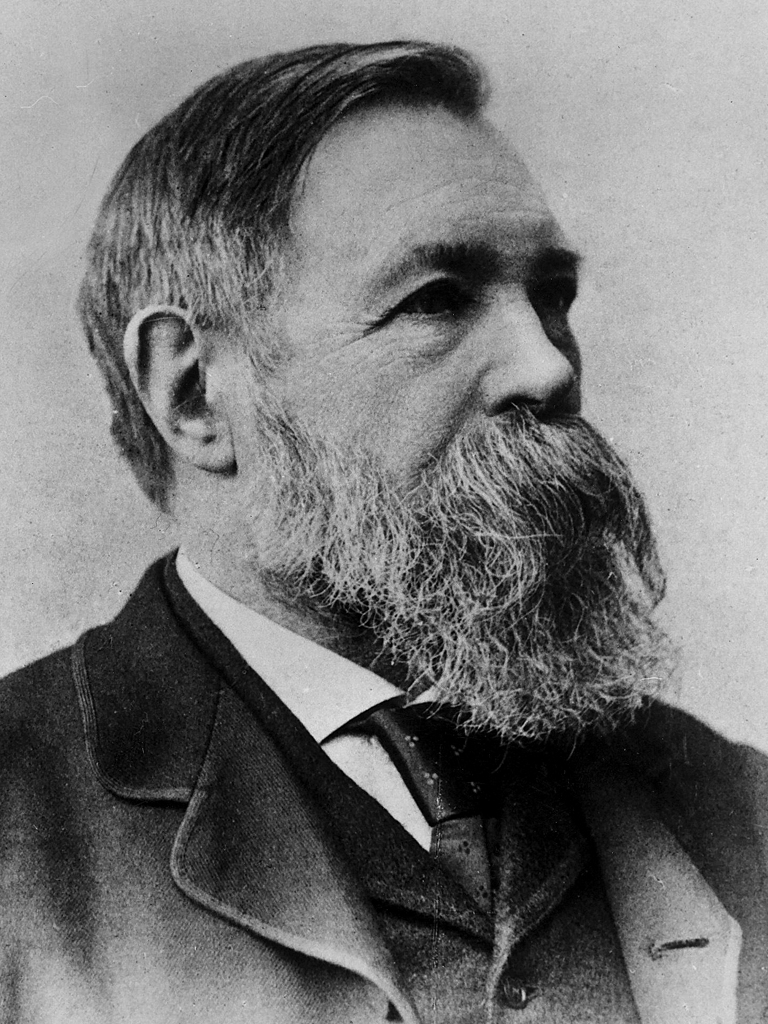
\includegraphics[width=50mm]{images/engels.jpg}
      \caption{エンゲルス} 
  \end{figure}


家族史〔の研究〕は、一八六一年、バッハオーフェンの『母権論』の刊行をもってはじまる。著者はここで以下の主張を提起する。(一)人類は当初、彼が娼婦制〔ヘテリスムス〕という誤った表現でよぶ無拘束の性的交渉の生活をおくっていたこと、(二)このような交渉は不正の確実さをすべて排除してしまうこと、したがって血統は女系によって{\——}母権によって{\——}しかたどれなかったこと、そしてこれは元来すべての古代民族にみられたこと、(三)その結果、女性には、若い世代の確実に知りうる唯一の親である母として、高度の尊敬と信望がはらわれ、バッハオーフェンの考えによれば、これは完全な女性支配(Gynaikokratie)にまで高められたこと、(四)女性が一人の男性に専属する一夫一婦制への移行は、太古の宗教戒律の侵害(すなわち、実際にはその女性にたいする他の男性たちの古来の要求権の侵害)を内包していて、この侵害をつぐなうか、またはその容認をあがなうかするには、時期をかぎっておこなわれる女性の肉体提供が必要であったこと、これである。(14)

\subsection*{}



母権制の転覆は、女性の世界史的な敗北であった。男性は家のなかでも舵をにぎり、女性は品位をけがされ、男性の情慾の奴隷、子供を生むたんなる道具となった。とくに英雄時代の、そしてそれにもまして古典時代のギリシャ人のばあいに公然と示されているような、女性のこのいやしめられた地位は、しだいに美化され、つつみ隠されて、ところによってはやや緩和された形態をまとったりもしたが、しかしそれはけっして除去されていない。

いまや樹立された男性の独裁の第一の結果は、この時期に姿を現わす家父長制家族という中間形態に示される。そのおもな特徴をなすものは、後述の一夫多妻制ではなくて、「多数の自由人と非自由人とを家長権力のもとに一家族に組織することである。セム人の形態では、この家長は一夫多妻の生活をおくり、非自由人は一人の妻と子をもち、そしてこの全組織の目的は、区分された領域で畜群の世話をすることである」〔モーガン、前掲書〔『古代社会』〕、下巻、二七〇頁〕。本質的な点は非自由人の包摂と家父権力であり、したがって、この家族形態の完成した型はローマの家族である。familia〔家族〕という言葉は、本来は、感傷と家庭不和とから構成される今日の俗物の理想を意味するのではない。ローマ人のばあいには、それは当初、けっして夫婦とその子供を指すのではなくて、奴隷だけを指す。famulusは家内奴隷のことであり、familiaは一人の男に属する奴隷の総体のことである。ガイウスの時代〔紀元二世紀〕になっても、familia, id est patrimonium(〔ファミリア〕すなわち相続分)は遺言によって遺贈されていた。この表現は、ローマ人が一つの新しい社会的な有機体を表示するために発明したものであって、この有機体の長は、妻子と多数の奴隷をローマ的家父権力のもとに従え、全員に対する生殺与奪の権利をもっていたのである。「したがってこの言葉は、ラテン諸部族の鉄甲がための家族制度よりも古いものではない。この家族制度は、畑地耕作と合法化された奴隷制とが採用されたのちに、そしてアーリア系イタリック人がギリシャ人から分離したのちに、現われたのである」〔モーガン、同書、二七七頁〕。マルクスはつけ加えていう。「近代的家族は、はじめから農耕のための労役と関係をもつから、たんに奴隷制(servitus)だけではなく農奴制をも、萌芽として含んでいる。それは、のちに社会とその国家のうちに広範に発展してくるすべての対立を、縮図として内包している」〔マルクス、前掲『ノート』五一頁〕。

このような家族形態は、対偶婚から単婚への移行を示している。妻の貞操を、したがって子の父性を確保するために、妻は夫の権力に無条件にゆだねられる。夫が妻を殺しても、それは彼が自分の権利を行使したいだけのことである。(75-77)

\subsection*{}




このようにして、婚姻には、全体として人類発展の三つの主要段階に照応する三つの主要形態がある。野蛮期には集団婚が、未開期には対偶婚が、文明期には姦通と売春によって補足される単婚が。対偶婚と単婚とのあいだには、未開の上位段階で、女奴隷にたいする男性の支配と一夫多妻制が割り込む。

われわれの全叙述が証明したように、この順序のうちに示される進歩は、女性が集団婚の性的自由をますます奪われてゆくのに、男性はそうではない、という特質と結びついている。そして実際に集団婚は、男性にとっては事実上今日まで存続している。女性のばあいには犯罪であり、重大な法律的および社会的な結果をともなうことが、男性のばあいには名誉とみなされたり、それほどでなくとも、最悪のばあいでも安んじて耐えられる軽微な道徳上の汚点としかみなされない。しかし、古来の娼婦制が現代において資本主義的商品生産によって変化させられ、それに適合させられればさせられるほど、そしてそれが露骨な売春に転化すればするほど、それはますます退廃的に作用する。しかしそれは、女性よりも男性をはるかにひどく退廃させる。売春は、女性のあいだでは、それに陥った不幸なものを堕落させるだけであり、これさえも、その程度はふつうに考えられるほどのものではけっしてない。これに反して、売春は全男性界の品位を低下させる。こうして、とくに男性の長期にわたる婚約状態は、十中の九までが婚姻上の不貞を学ぶ正式の予備校なのである。

いまやわれわれは、一つの社会的変革にむかって進んでおり、そこでは、単婚のこれまでの経済的基礎が、その補足物である売春のそれと同様に、確実に消滅するであろう。単婚は、比較的大きな富の一人の手{\——}しかも夫の手{\——}への集中と、この富を他人ではなしにこの夫の子供たちに相続させようとする欲望とから成立した。そのために、夫のではなしに妻の単婚が必要とされたのであり、したがってこの妻の単婚は、夫の公然または隠然の多妻制をけっして妨げるものではなかった。しかし、きたるべき社会的変革は、すくなくとも耐久的な相続可能な富{\——}生産手段{\——}のかぎりなく大きな部分を社会的所有に転化することによって、このような相続にかんするすべての配慮を最小限のものに縮小するであろう。ところで、単婚は経済的諸原因から成立したのであるから、これらの原因が消滅すれば、単婚も消滅するであろうか。

それは消滅しないばかりか、むしろはじめて完全に実現されるであろう、と答えても不当ではあるまい、なぜなら、生産手段の社会的所有への転化とともに、賃労働、プロレタリアートもまた消滅し、したがって、一定の{\——}統計的に計算できる{\——}数の女性にとって、貨幣〔かね〕と引換えに自分の肉体を提供する必要もまた消滅するからである。売春は消滅するが、単婚は没落するかわりに、ついに{\——}男性にとってもまた現実となる。

したがって、男性の地位はいずれにしても大きく変えられる。しかし女性の、すべての女性の地位もまた、いちじるしい変更をこうむる。生産手段の共同所有への移行とともに、個別家族は社会の経済的単位であることをやめる。私的家計は一つの社会的産業に転化する。子供たちの養育や教育は公的な事項となる。嫡出子であろうと私生児であろうと、一様にすべての子供の世話を社会がみる。これによって、今日、娘が恋人に思いきって身をまかせるのを妨げる、もっとも本質的な社会的{\——}道徳的ならびに経済的{\——}要因をなしているところの、「結果」にたいする心配がなくなる。このことは、いっそう無遠慮な性交を、したがってまた処女の誇りや女の恥についてのいっそうルーズな世論を、しだいに生じさせるのに十分な原因となるのではなかろうか。そして最後に、近代世界では単婚と売春がなるほど対立物ではあるが、しかし不可分の対立物、同一の社会状態の両極であることは、すでにわれわれのみたところではなかったろうか。売春は、単婚を道づれにしないで消滅できるのだろうか。(98-100)







%%% Local Variables:
%%% mode: japanese-latex
%%% TeX-master: "main_gendai"
%%% coding: utf-8
%%% End:
